\documentclass[12pt]{extarticle}
%Some packages I commonly use.
\usepackage[portuguese]{babel}
\usepackage{graphicx}
\usepackage{framed}
\usepackage[normalem]{ulem}
\usepackage{amsmath}
\usepackage{amsthm}
\usepackage{amssymb}
\usepackage{amsfonts}
\usepackage{enumerate}
\usepackage[utf8]{inputenc}
\usepackage{float}
\usepackage{gensymb}
\usepackage[top=1 in,bottom=1in, left=1 in, right=1 in]{geometry}
\usepackage{multirow}
\usepackage{caption}
\usepackage{subcaption}
\usepackage[utf8]{inputenc}

%A bunch of definitions that make my life easier
\newcommand{\matlab}{{\sc Matlab} }
\newcommand{\cvec}[1]{{\mathbf #1}}
\newcommand{\rvec}[1]{\vec{\mathbf #1}}
\newcommand{\ihat}{\hat{\textbf{\i}}}
\newcommand{\jhat}{\hat{\textbf{\j}}}
\newcommand{\khat}{\hat{\textbf{k}}}
\newcommand{\minor}{{\rm minor}}
\newcommand{\trace}{{\rm trace}}
\newcommand{\spn}{{\rm Span}}
\newcommand{\rem}{{\rm rem}}
\newcommand{\ran}{{\rm range}}
\newcommand{\range}{{\rm range}}
\newcommand{\mdiv}{{\rm div}}
\newcommand{\proj}{{\rm proj}}
\newcommand{\R}{\mathbb{R}}
\newcommand{\N}{\mathbb{N}}
\newcommand{\Q}{\mathbb{Q}}
\newcommand{\Z}{\mathbb{Z}}
\newcommand{\<}{\langle}
\renewcommand{\>}{\rangle}
\renewcommand{\emptyset}{\varnothing}
\newcommand{\attn}[1]{\textbf{#1}}
\theoremstyle{definition}
\newtheorem{theorem}{Theorem}
\newtheorem{corollary}{Corollary}
\newtheorem*{definition}{Definition}
\newtheorem*{example}{Example}
\newtheorem*{note}{Note}
\newtheorem{exercise}{Exercise}
\newcommand{\bproof}{\bigskip {\bf Proof. }}
\newcommand{\eproof}{\hfill\qedsymbol}
\newcommand{\Disp}{\displaystyle}
\newcommand{\qe}{\hfill\(\bigtriangledown\)}
\setlength{\columnseprule}{1 pt}
\usepackage[utf8]{inputenc}

\title{Plano Inclinado - Partes 1 e 2}
\author{Felipe Salvador}
\date{Atualizado em \today}

\begin{document}

\maketitle

\section{Introdução}

Nessa aula, veremos como é a física por trás de blocos em planos inclinados como ladeiras. Analisaremos os problemas com diversas forças envolvidas, além de desenvolver técnicas de resolução dos problemas para diversas formas. Em especial, iremos tratar de 4 problemas:
\begin{enumerate}
    \item Bloco num plano inclinado liso (sem atrito) sob ação da gravidade;
    \item Bloco num plano inclinado rugoso (com atrito) sob ação da gravidade;
    \item Bloco acoplado a uma mola fixa num plano inclinado liso (sem atrito) sob ação da gravidade;
    \item Bloco acoplado a uma mola fixa num plano inclinado rugoso (com atrito) sob ação da gravidade;
\end{enumerate}

\section{Bloco num plano inclinado liso (sem atrito) sob ação da gravidade}

Nesse problema, nós iremos analisar os problemas de que um bloco parado ou em movimento num plano inclinado por um ângulo $\theta$. Para fazer o plano e o problema, vamos pensar num bloco sobre uma cunha, cuja face diagonal tem angulação $\theta$. A seguir está o diagrama de forças no bloco:
\begin{figure}[H]
    \centering
    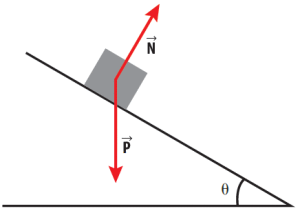
\includegraphics[width=0.3\textwidth]{screenshot_66.png}
    \label{fig:inclinado_1}
\end{figure}

Para a gente poder fazer a análise, precisamos escolher um sistema de coordenadas. É claro que podemos escolher o sistema de coordenadas em que a direção vertical é o eixo 'y' e a direção horizontal é o eixo 'x'. Mas isso não seria conveniente, porque o bloco irá se movimentar verticalmente (vai cair) e também irá para direita.

O ideal é escolhermos um sistema de coordenadas tal que o movimento só ocorre numa única direção. Isso é possível se escolhermos o eixo x na direção paralela à face diagonal da cunha e o eixo y na direção perpendicular à face diagonal da cunha. Assim, como o bloco se movimenta paralelamente à face diagonal, o bloco só se move na direção x.

Isso faz com que o problema se torne mais fácil de se resolver e, de tabela, alinhamos a força normal com o eixo y (pois, \textbf{a força normal é sempre perpendicular à superfície que o corpo está}). Agora, o problema é que força peso não está numa direção de um dos eixos. Para resolver isso, usaremos a técnica de \textbf{decompor um vetor}.

A ideia por trás é que a força peso pode ser escrita pela soma de vetores, de forma que um vetor estará na direção do eixo y, enquanto o outro vetor da soma estará na direção do eixo x. Para ilustrar como funciona, veja a figura a seguir:

\begin{figure}[H]
    \centering
    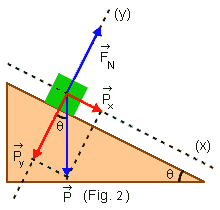
\includegraphics[width=0.5\textwidth]{_2025_38.png}
    \caption{Diagrama de forças sobre o bloco, em que decompomos a força peso como a soma de vetores: um na direção do eixo y e outro na direção do eixo x. Perceba também a escolha do sistema de coordenadas, conforme discutido acima.}
    \label{fig:decompose}
\end{figure}

Uma das questões importantes é saber o tamanho de cada vetor. Se olharmos os vetores $\vec{P}_x,\, \vec{P}_y\,e\, \vec{P}$, eles formam um triângulo retângulo. Por análise geométrica, o ângulo entre $\vec{P}_y$ e $\vec{P}$ é o mesmo ângulo da inclinação do plano: $\theta$.

Agora, vendo que os $\vec{P}_x,\, \vec{P}_y\,e\, \vec{P}$ fazem um triângulo retângulo, podemos usar as relações trigonométricas para descrever as quantidades. Lembrando que os eixos x e y fazem $90^\circ$ entre si, então $\vec{P}_x\, e \, \vec{P}_y$ fazem $90^\circ$. Dessa forma, $\vec{P}$ é a hipotenusa, o cateto oposto é o $\vec{P}_x$ e o cateto adjacente é o $\vec{P}_y$.

Com isso e o uso das relações de trigonometria, podemos determinar os módulos dos vetores $\vec{P}_x\, e \, \vec{P}_y$:
\begin{align*}
    \cos\theta = \frac{P_y}{P} \implies P_y =\cos\theta P
\end{align*}
\begin{equation}\label{eq:p_y}
    P_y = mg\cos\theta
\end{equation}

\begin{align*}
    sen\,\theta = \frac{P_x}{P} \implies P_x = P\,sen\,\theta
\end{align*}
\begin{equation}\label{eq:p_x}
    P_x = mg\,sen\,\theta
\end{equation}

Na figura abaixo, está denotado o diagrama com os valores das forças $\vec{P}_x\, e \, \vec{P}_y$, decompostas da força peso.
\begin{figure}[H]
    \centering
    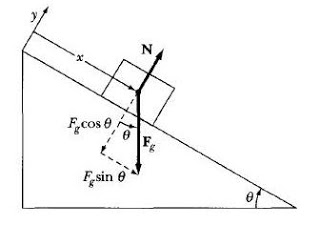
\includegraphics[width=0.5\textwidth]{imagem01.JPG}
    \label{fig:decompose_2}
\end{figure}

Com isso, agora podemos finalmente analisar as forças envolvidas, uma vez que não temos mais forças apontando para direções diferentes dos eixos x e y.

Em relação ao eixo y, percebemos que o bloco não irá se mover, uma vez ele não sobe nem desce em relação à superfície do plano. Por isso, a força resultante na direção y é:
\begin{align*}
    (F_r)_y =0
\end{align*}

Mas, na direção do eixo y, temos 2 forças atuantes: a força normal $\vec{N}$ (no sentido positivo do eixo) e a força peso decomposta no eixo y $\vec{P}_y$ (no sentido negativo do eixo). Por isso:
\begin{align*}
    (F_r)_y = N - P_y
\end{align*}
Só que pela equação (\ref{eq:p_y}), temos a relação do módulo da força $P_y$:
\begin{align*}
    0=(F_r)_y = N - mg\cos\,\theta
\end{align*}
Logo:
\begin{equation}
    N = mg\cos\,\theta
\end{equation}

Dessa forma, a força normal que o corpo sente num plano inclinado é a força peso vezes um fator $\cos\theta$, que carrega a dependência do ângulo do plano. Como uma forma de checar se o nosso resultado é consistente é tomar o ângulo $\theta=0$ (o que seria um plano horizontal). Como $\cos 0 =1$, teremos: $N = mg$ - que é o resultado que obtemos nas aulas sobre Leis de Newton.

Agora, na direção do eixo x, temos só uma força atuante: a força peso decomposta no eixo x$\vec{P}_x$ (no sentido positivo do eixo). Com isso, aplicando a expressão da equação (\ref{eq:p_x}), a força resultante na direção do eixo x:
\begin{equation}
    (F_r)_x = P_x = mg\,sen\,\theta
\end{equation}
Aplicando a Segunda Lei de Newton, a aceleração que um corpo no plano inclinado liso sofre é:
\begin{equation}
    m\,a_x = (F_r)_x = mg\,sen\,\theta \implies \boxed{a_x = g\,sen\,\theta}
\end{equation}

Ou seja, um corpo num plano inclinado sofre uma aceleração igual à aceleração da gravidade vezes um fator $sen\,\theta$, que carrega a dependência do angulação do plano inclinado. Para checar consistência, vamos para o caso de um plano horizontal, que é quando $\theta=0$. Como $sen\,0=0$, a aceleração no eixo x é: $a_x = g\,sen\,0 = 0$, logo o corpo não ganha/perde velocidade no plano horizontal liso. 

O que faz sentido, porque se não há forças horizontais sendo aplicadas (até porque $P_x=mg\,sen\,\theta =0$ também), o corpo vai continuar na inercia (seja em movimento retilíneo uniforme ou parado).]

\textbf{Quero levantar um ponto importante: em nenhum momento tomamos suposições sobre a velocidade inicial do corpo (se ele estava parado ou em movimento). Então, os resultados obtidos são gerais e válidos para os 2 casos - corpo inicialmente parado e corpo já em movimento.} 

Levanto atenção também, para o caso de um corpo que tenha velocidade inicial negativa na direção do eixo x ($v_{0x} < 0$), ou seja, "subindo a ladeira". Para esse caso, o corpo irá subir, até perder toda a velocidade (pois a aceleração na direção x é positiva, como vimos) e depois esse corpo começa a "descer a ladeira".

\textit{Exemplo:} Um bloco de massa de 2 kg é posto em repouso num plano com inclinação de $\theta=30^\circ$. A partir de t=0s, o bloco é solto. Qual é a aceleração que o bloco sofre? Qual é o valor da força normal? 

(\textit{Note e adote: $g=10m/s^2$, $sen\,30^\circ = 1/2$ e $\cos30^\circ = \sqrt{3}/2$})
\begin{figure}[H]
    \centering
    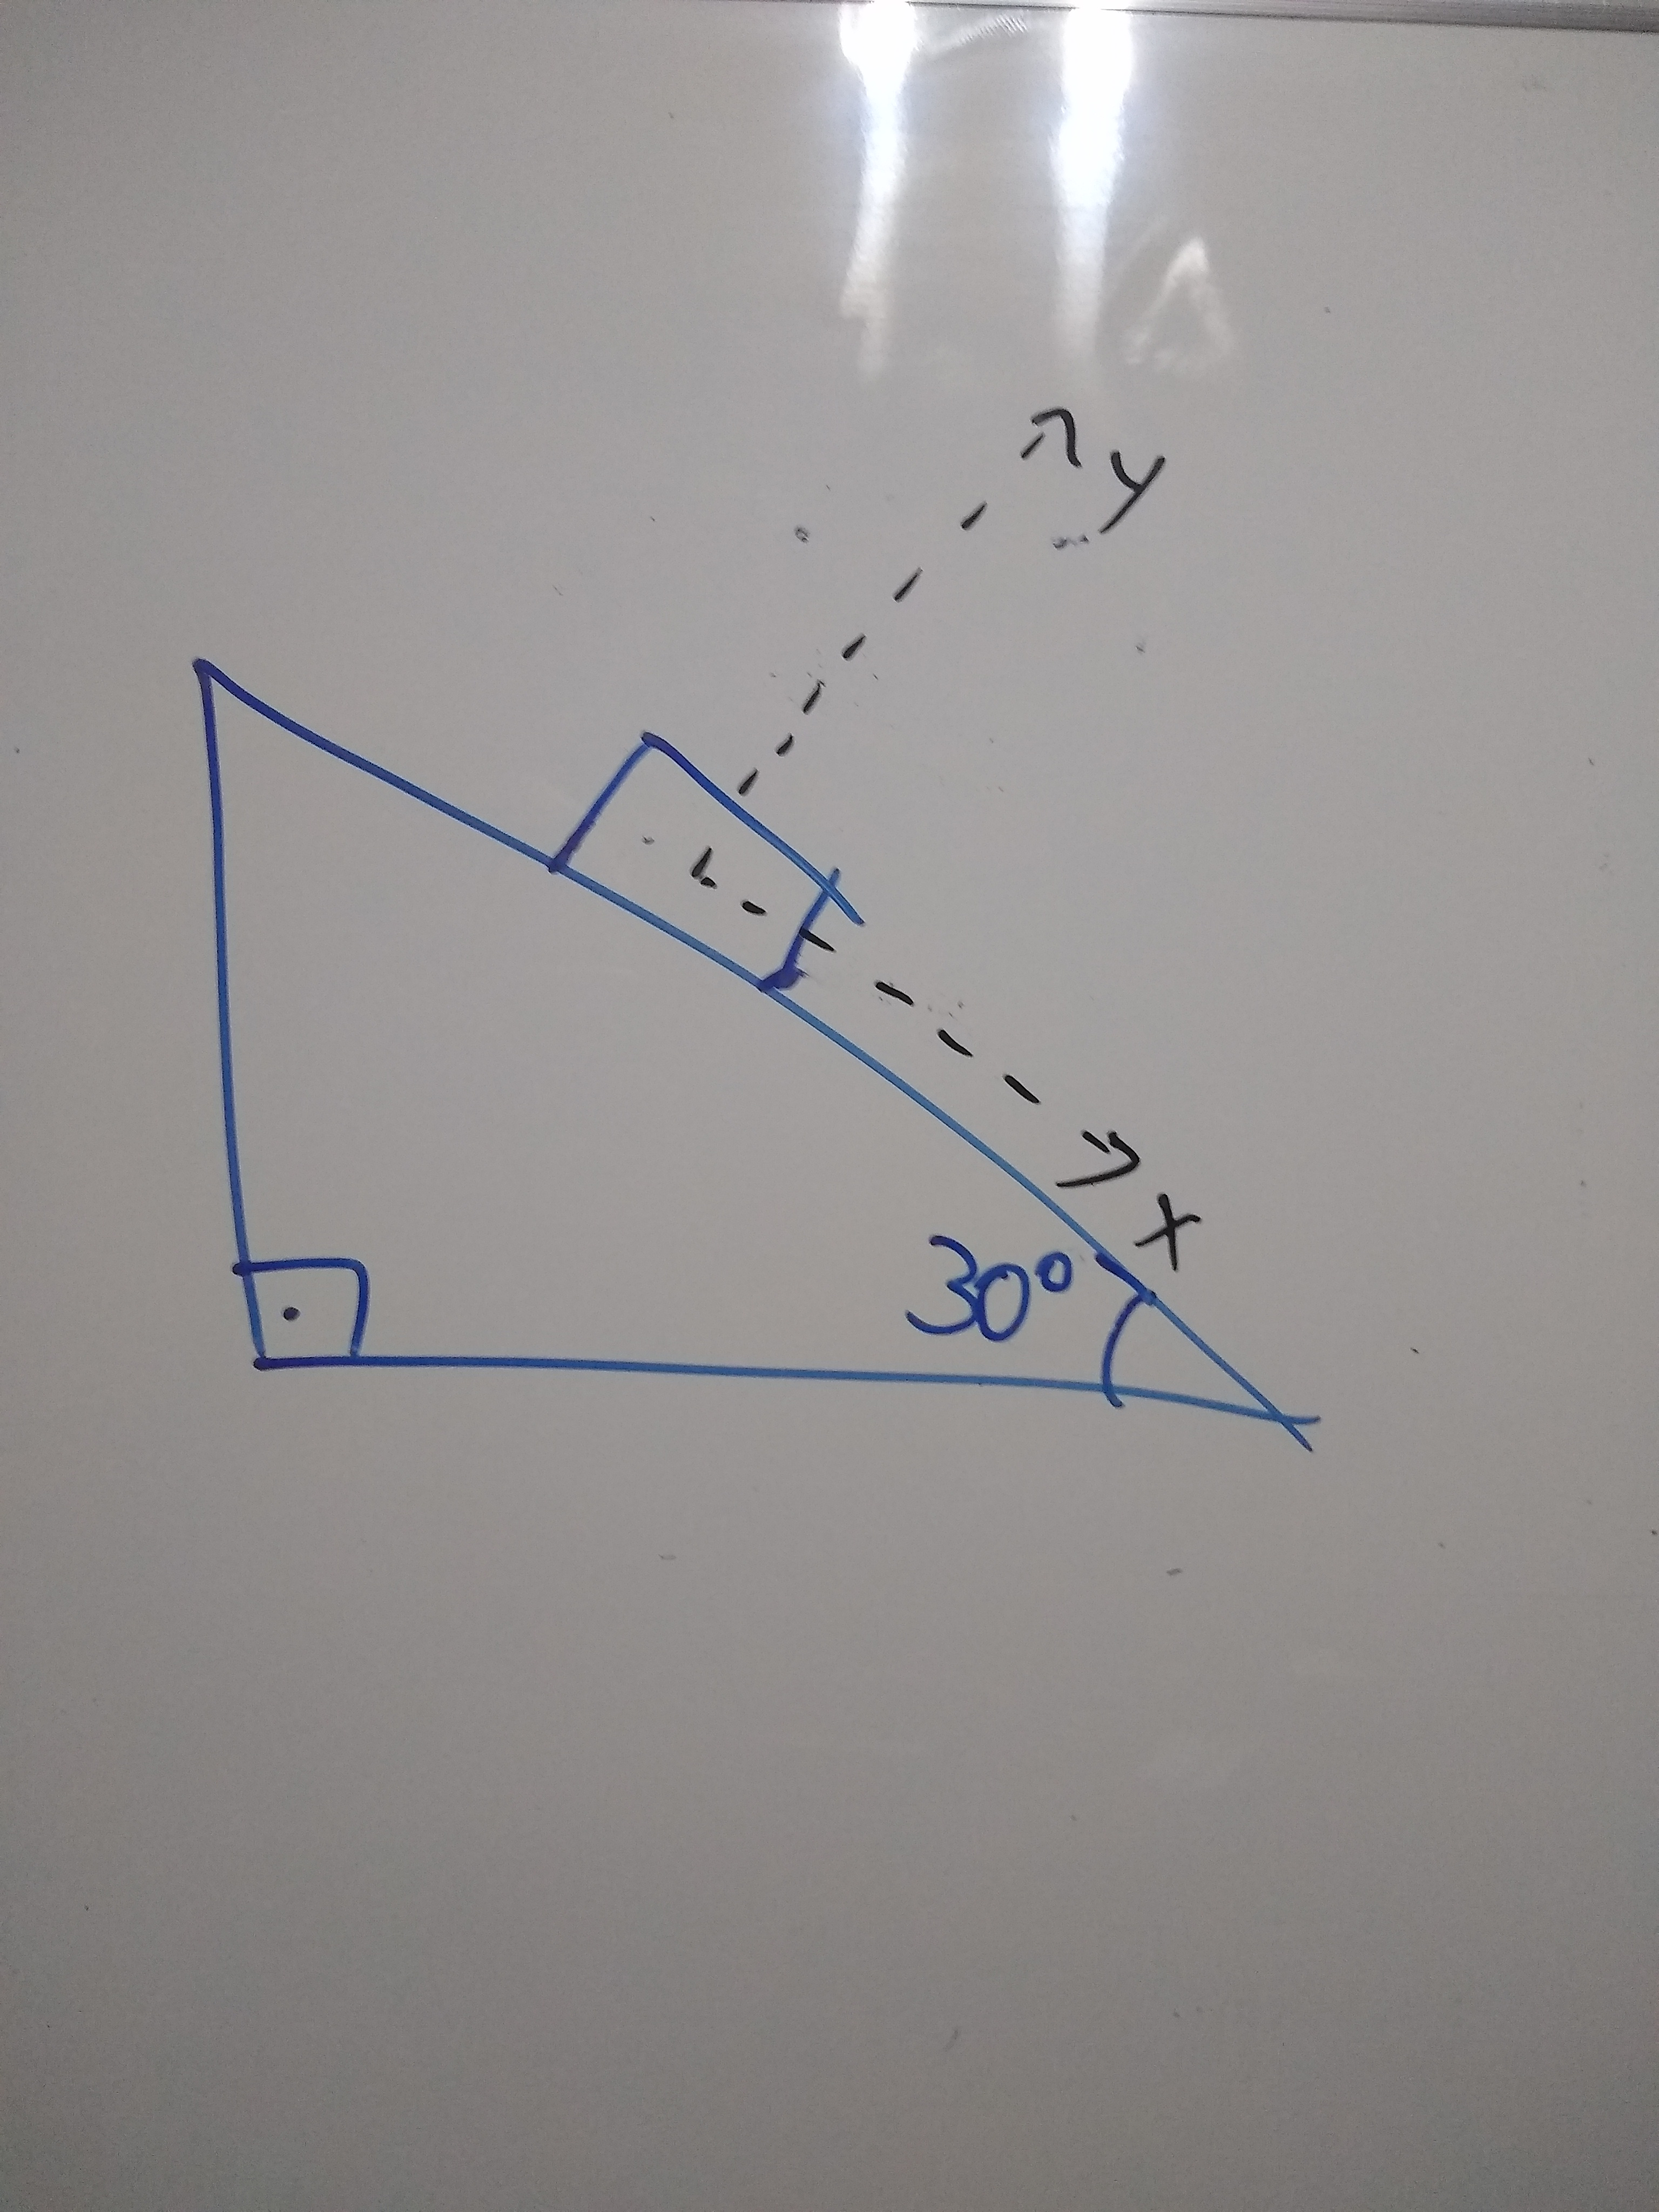
\includegraphics[width=0.3\textwidth]{IMG_20200602_002611925.jpg}
    \label{fig:ex_1}
\end{figure}

Aqui a gente usa os princípios descritos acima: A força peso é decomposta na direção y ($P_y=mg\cos\theta$) e na direção x ($P_x=mg\,sen\,\theta$). Lembrar que a força normal é na direção y, pois ela é sempre perpendicular à superfície. No nosso problema, $\theta =30^\circ$, então a força resultante será:
\begin{align*}
    0=(F_r)_y &= N - P_y = N - mg\cos\theta\\
    (F_r)_x &= P_x = mg\,sen\,\theta
\end{align*}
(lembrando que como o bloco está inicialmente em contato com a superfície do plano e não se movimenta na direção y durante o movimento, por isso a força resultante em y é 0.) Com isso, aplicando a Segunda Lei de Newton para a direção x:
\begin{align*}
    N &= mg\cos\theta\\
    m\,a_x&= (F_r)_x = mg\,sen\,\theta
\end{align*}
Aplicando os valores dados:
\begin{align*}
    N &= 2*10*\cos30^\circ = 20*\frac{\sqrt{3}}{2} \implies N = 10\sqrt{3}\, N\\
    &2\,a_x = 2*10\,sen\,30^\circ \implies a_x = 10*\frac{1}{2} \implies a_x = 5\,m/s^2
\end{align*}
\section{Bloco num plano inclinado rugoso (com atrito) sob ação da gravidade}

A partir dessas seções, nós iremos adicionar outras forças que vimos na aula passada, todavia o procedimento que iremos tomar é o mesmo da seção anterior: 
\begin{enumerate}
    \item Escolher o sistema de coordenadas de forma que o movimento só acontece em uma direção (O eixo y perpendicular à superfície diagonal e o eixo x paralelo à superfície diagonal);
    \item Decompor a força Peso nas direções dos eixos, calculando as suas componentes;
    \item Calcular, em cada direção (x e y), a força resultante;
    \item Aplicar a Segunda Lei de Newton para cada direção.
\end{enumerate}

Toda discussão sobre as forças já está na seção anterior, então caso algo não fique claro, volte na seção anterior e releia. Aqui a novidade é a existência de uma força de atrito. Vamos separar o problema em 2 subproblemas.
\subsection{Bloco num plano inclinado rugoso (com atrito) sob ação da gravidade - caso estático}

Nesse caso, o bloco não se movimenta, ele fica parado. Isso é possível, pois sabemos que a força de atrito atua na direção contrária ao movimento (no caso dinâmico) ou na direção contrária à tendência de movimento (no caso estático). Como o corpo se movimenta/tem tendência a se movimentar na direção x positiva, então \textbf{a força de atrito está atuando na direção x negativa.}

Com isso, o diagrama de forças no corpo é o a seguir:
\begin{figure}[H]
    \centering
    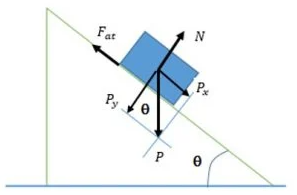
\includegraphics[width=0.5\textwidth]{atrito_estatico.png}
    \label{fig:atrito_estatico}
\end{figure}

Para esse caso estático, a condição que temos que respeitar é a seguinte:
\begin{equation}
    (F_r)_x = (F_r)_y = 0
\end{equation}
\noindent ou seja, as forças resultantes nas direções x e y tem que ser 0. Por isso na direção y, temos que:
\begin{align*}
    (F_r)_y &= N - P_y =0\\
    &= N - mg\cos\theta
\end{align*}
\begin{equation}
    N = mg\cos\theta
\end{equation}
E na direção x:
\begin{align*}
    (F_r)_x &= P_x - F_{at}=0 \\
    &= mg\,sen\,\theta - F_{at} =0
\end{align*}
\begin{equation}
    F_{at} = mg\,sen\,\theta
\end{equation}

Caso o exercício fale que a força de atrito é máxima (o que significa que é o máximo que o atrito consegue segurar no caso estático, mais do que isso o objeto começa a se mover), podemos usar a fórmula da força de atrito:
\begin{align*}
    F_{at} = \mu\,N
\end{align*}
Como vimos, $N=mg\cos\theta$, então:
\begin{align*}
    \mu\,N = F_{at} &= mg\,sen\,\theta\\
    \mu\,mg\cos\theta &= mg\,sen\,\theta
\end{align*}
\begin{equation}
    \boxed{\mu = \frac{sen\,\theta}{\cos\theta} = \tan\theta}
\end{equation}

Ou seja, o coeficiente de atrito limite para um bloco parado é igual à tangente do angulação do plano, no caso em que a força de atrito estático é a limite.

\textit{Exemplo:} Um bloco de 10 kg permanece parado num plano rugoso. O plano tem inclinação de $37^\circ$. Calcule a força de atrito que está sendo aplicada nesse bloco.

\textit{Note e adote: $g=10\,m/s^2$, $sen\,37^\circ = 0,6$ e $\cos37^\circ =0,8$}
\begin{figure}[H]
    \centering
    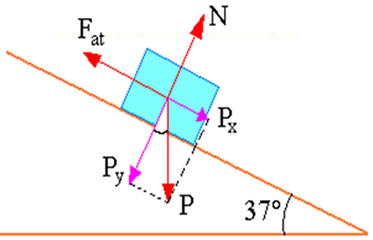
\includegraphics[width=0.4\textwidth]{resposta-exercicio-3.jpg}
    \caption{Esquema de forças do exemplo}
    \label{fig:ex_2}
\end{figure}

A figura dada já fez a decomposição da força peso para a gente, só basta calcular cada componente:
\begin{align*}
    P_y &= mg\cos\theta = 10*10*0,8 = 80\, N\\
    P_x &=mg\,sen\,\theta = 10*10*0,6 = 60\,N
\end{align*}
Agora, vamos calcular a força resultante de para cada direção, lembrando que como o bloco permanece parado no espaço, então, a força resultante nas duas direções são 0.
\begin{align*}
    0=(F_r)_x &= P_x - F_{at} = 60 - F_{at} \implies F_{at} = 60\,N\\
    0=(F_r)_y &= N -P_y = N -80 \implies N = 80\,N\\
\end{align*}

\subsection{Bloco num plano inclinado rugoso (com atrito) sob ação da gravidade - caso dinâmico}

A "receita de bolo" a ser seguida é a mesma da parte anterior. A diferença agora é que para o caso dinâmico, a fórmula da força de atrito é:
\begin{align*}
    F_{at}=\mu_c\,N
\end{align*}
\noindent em que $\mu_c$ é o coeficiente de atrito dinâmico e 'N' é a força normal.

Diferentemente do caso estático, agora o bloco se move na direção x e podemos determinar a aceleração que esse bloco sofre.

\textit{Exemplo:} Dado um bloco de massa 5 kg sobre um plano com atrito. O plano tem uma inclinação de $37^\circ$. Sabendo que após $t=0$, o bloco é solto e começa a se movimentar, calcule a aceleração que ele sofre.

\textit{Note e adote: $g=10\,m/s^2$, $\mu_c=0,2$, $sen\,37^\circ = 0,6$ e $\cos37^\circ =0,8$}

O esquema de forças é idêntico ao da figura (\ref{fig:ex_2}), então vamos reusá-lo. Calculando a cada componente da força peso decomposta:
\begin{align*}
    P_x &= 5*10*0,6 = 30\,N\\
    P_y &= 5*10*0,8 = 40\,N
\end{align*}
Agora, vamos calcular a força resultante em cada direção:
\begin{align*}
    (F_r)_x &= P_x - F_{at} = 30 - \mu*N \\
    (F_r)_y &= N - P_y = N - 40
\end{align*}
Como sabemos que o corpo não se movimenta na direção do eixo y, então a força resultante em y é 0. Logo: $0 = N -40 \implies N =40\,N$

Com isso, podemos calcular a força de atrito e a força resultante em x:
\begin{align*}
    (F_r)_x = 30 -0,2*40 = 30 -8 \implies (F_r)_x = 22\,N
\end{align*}

Usando a Segunda Lei de Newton para achar a aceleração:
\begin{align*}
    m\,a_x = (F_r)_x \implies 5\,a_x = 22 \implies a_x = 4,4\,m/s^2
\end{align*}

\section{Bloco acoplado a uma mola fixa num plano inclinado liso (sem  atrito) sob ação da gravidade}

Nessa parte, iremos adicionar o efeito de uma mola segurando o objeto num plano inclinado. Lembremos que a força produzida por uma mola é dada por:
\begin{equation}
    F_{el} = k\Delta x
\end{equation}
em que $\Delta x$ é a deformação de uma mola. É importante ressaltar que o sentido da força é \textbf{contrário} ao sentido da deformação, então se a mola estiver sendo esticada, a força será para puxar e vice-versa.

O problema pode ser descrito dessa forma:
\begin{figure}[H]
    \centering
    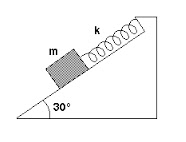
\includegraphics[width=0.4\textwidth]{Pic-Hooke-04.jpg}
    \caption{Arranjo do sistema de um bloco conectado a uma mola num plano inclinado}
    \label{fig:my_label}
\end{figure}

As forças desse problema são 3:
\begin{itemize}
    \item \textbf{A força Peso (P)} na vertical para baixo - $P=mg$
    \item \textbf{A força Normal (N)} na direção perpendicular à superfície que está o bloco
    \item \textbf{A força elástica ($F_{el}$)} na direção paralela à superfície (que no exemplo da figura, o sentido da força é subindo o bloco)  - $F_{el} = k\Delta x$
\end{itemize}

O diagrama de forças está a seguir:
\begin{figure}[H]
    \centering
    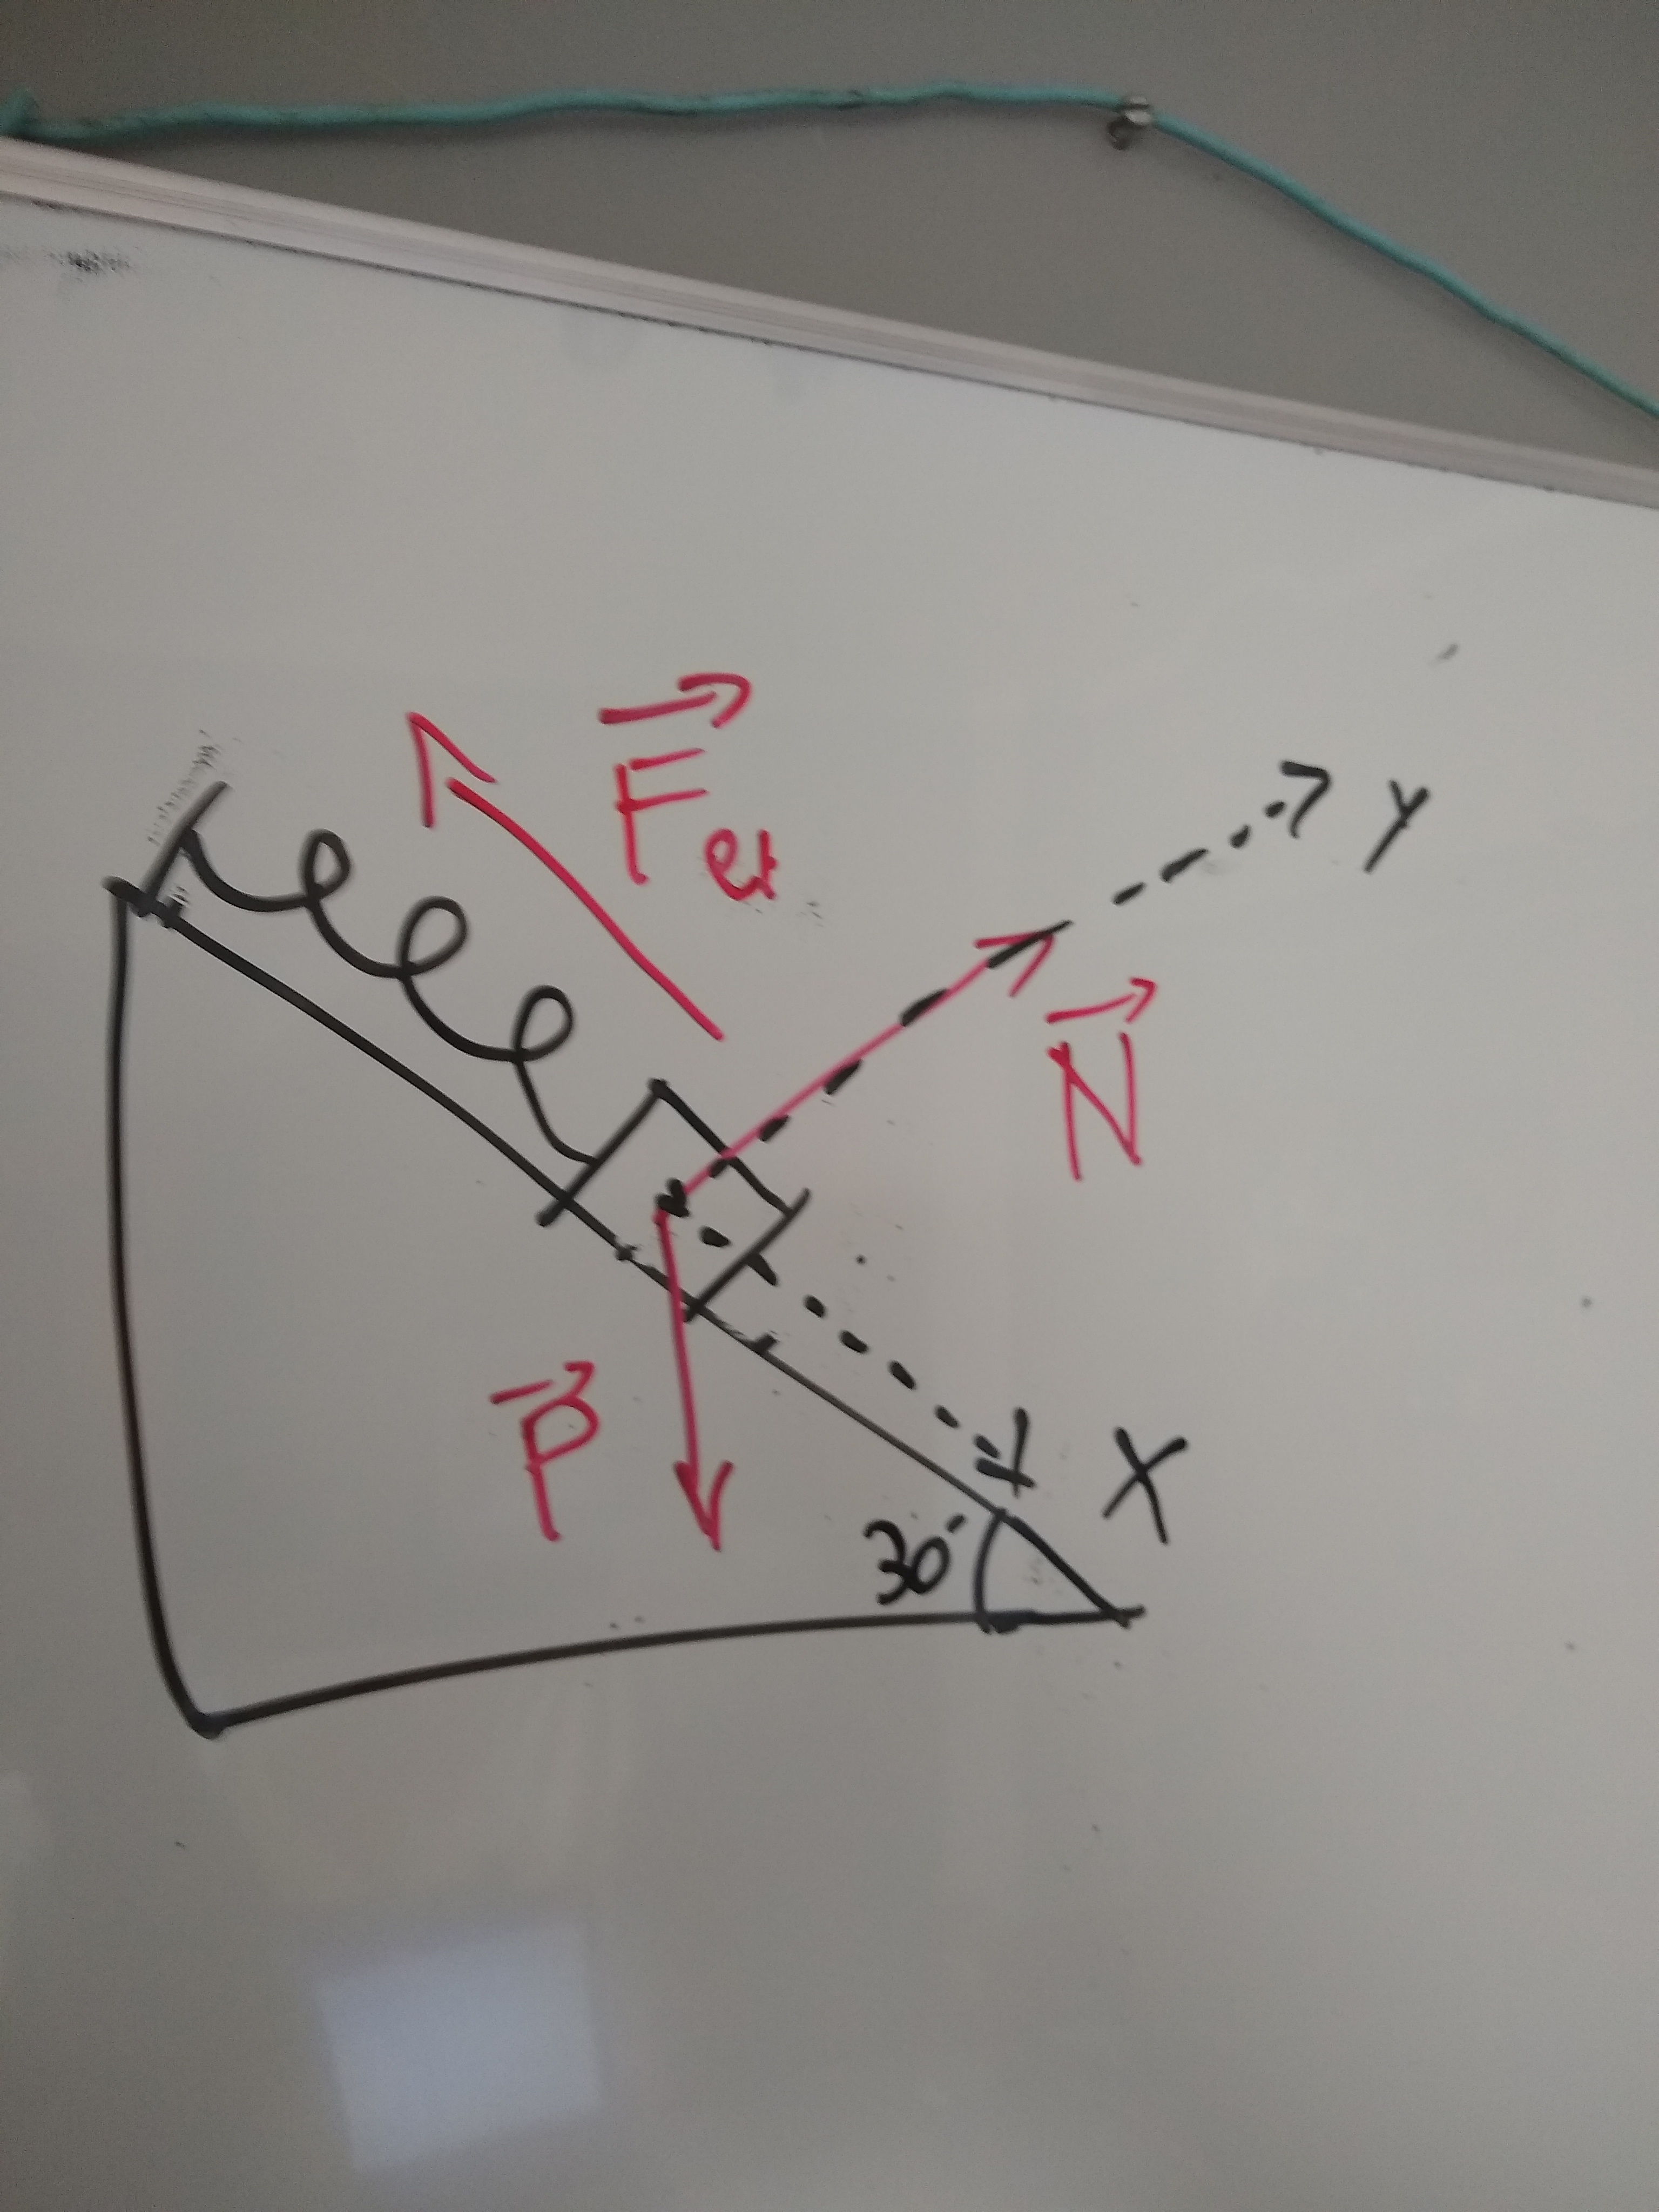
\includegraphics[width=0.4\textwidth]{plano_inclinado_mola.jpg}
    \caption{Diagrama de forças}
    \label{fig:mola_sem_atrito}
\end{figure}

Novamente, vamos decompor a força peso nas direções x e y (tomando $\theta=30^\circ$):
\begin{align*}
    &P_x = mg\,sen\,\theta \\
    &P_y = mg\,\cos\theta
\end{align*}

Com isso, podemos a força resultante em cada direção é:
\begin{align*}
    &(F_{res})_x = P_x - F_{el}\\
    &(F_{res})_y = N - P_y = 0 \implies N = mg\cos\theta
\end{align*}
\noindent em que força resultante na direção y tem que ser 0, porque o bloco não se movimenta nessa direção. Nesse problema, um caso interessante de analisar é encontrar a deformação da mola que faz com que o bloco fique parado no plano inclinado. Isso acontece quando as força elástica anula a força peso decomposta no eixo x:
\begin{align*}
    &P_x - F_{el} =0 \implies mg\,sen\,\theta = kx\\
    & \boxed{x = \frac{mg\,sen\,\theta}{k}}
\end{align*}

\textit{Exemplo:} Um bloco de 2kg é solto no topo de um plano inclinado com o ângulo de 30$^\circ$. Na base do plano, tem uma mola de constante $k=20\,N/m,$ para amortecer o bloco, conforme a figura abaixo:
\begin{figure}[H]
    \centering
    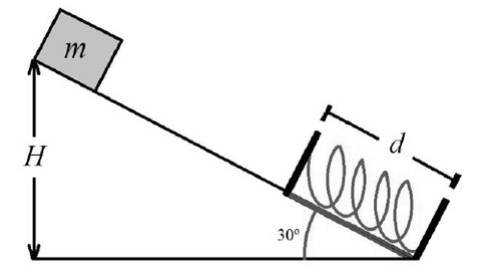
\includegraphics[width=0.4\textwidth]{forum11.jpg}
    \label{fig:ex_mola}
\end{figure}

Ao fim do movimento, o bloco está parado em contato com a mola, ache a deformação da mola. \textit{Note e adote: $g=10\,m/s^2$, $sen\,30^\circ = 1/2$ e $\cos30^\circ = \sqrt{3}/2$}

Como o exercício só quer a deformação, vamos só lidar com a direção x da força resultante. Fazendo o diagrama de forças igual ao da teoria acima, vemos que a força resultante em x é dada por:
\begin{align*}
    &(F_{res})_{x} = P_x - F_{el} =0\\
    &P_x = F_{el}\\
    &mg\,sen\,30^\circ = k\,x
\end{align*}
Colocando os valores:
\begin{equation*}
    2*10*\frac{1}{2} = 20*x \implies x= 0,5\, m
\end{equation*}

\section{Bloco acoplado a uma mola fixa num plano inclinado rugoso (com  atrito) sob ação da gravidade}

Para finalizar, vamos acrescentar o atrito à conta do plano inclinado com um bloco conectado à uma mola fixa. Sabemos que a força de atrito é dada por:
\begin{equation*}
    F_{at} = \mu\,N
\end{equation*}
\noindent em que $\mu$ é o coeficiente de atrito e $N$ é o módulo da força normal. Lembremos que a força de atrito ela atua na direção contrária ao movimenta ou na direção contrária à tendência de movimento. E que essa fórmula é somente para o atrito cinético ou para o atrito estático limite.

O diagrama de forças é a figura a seguir:
\begin{figure}[H]
    \centering
    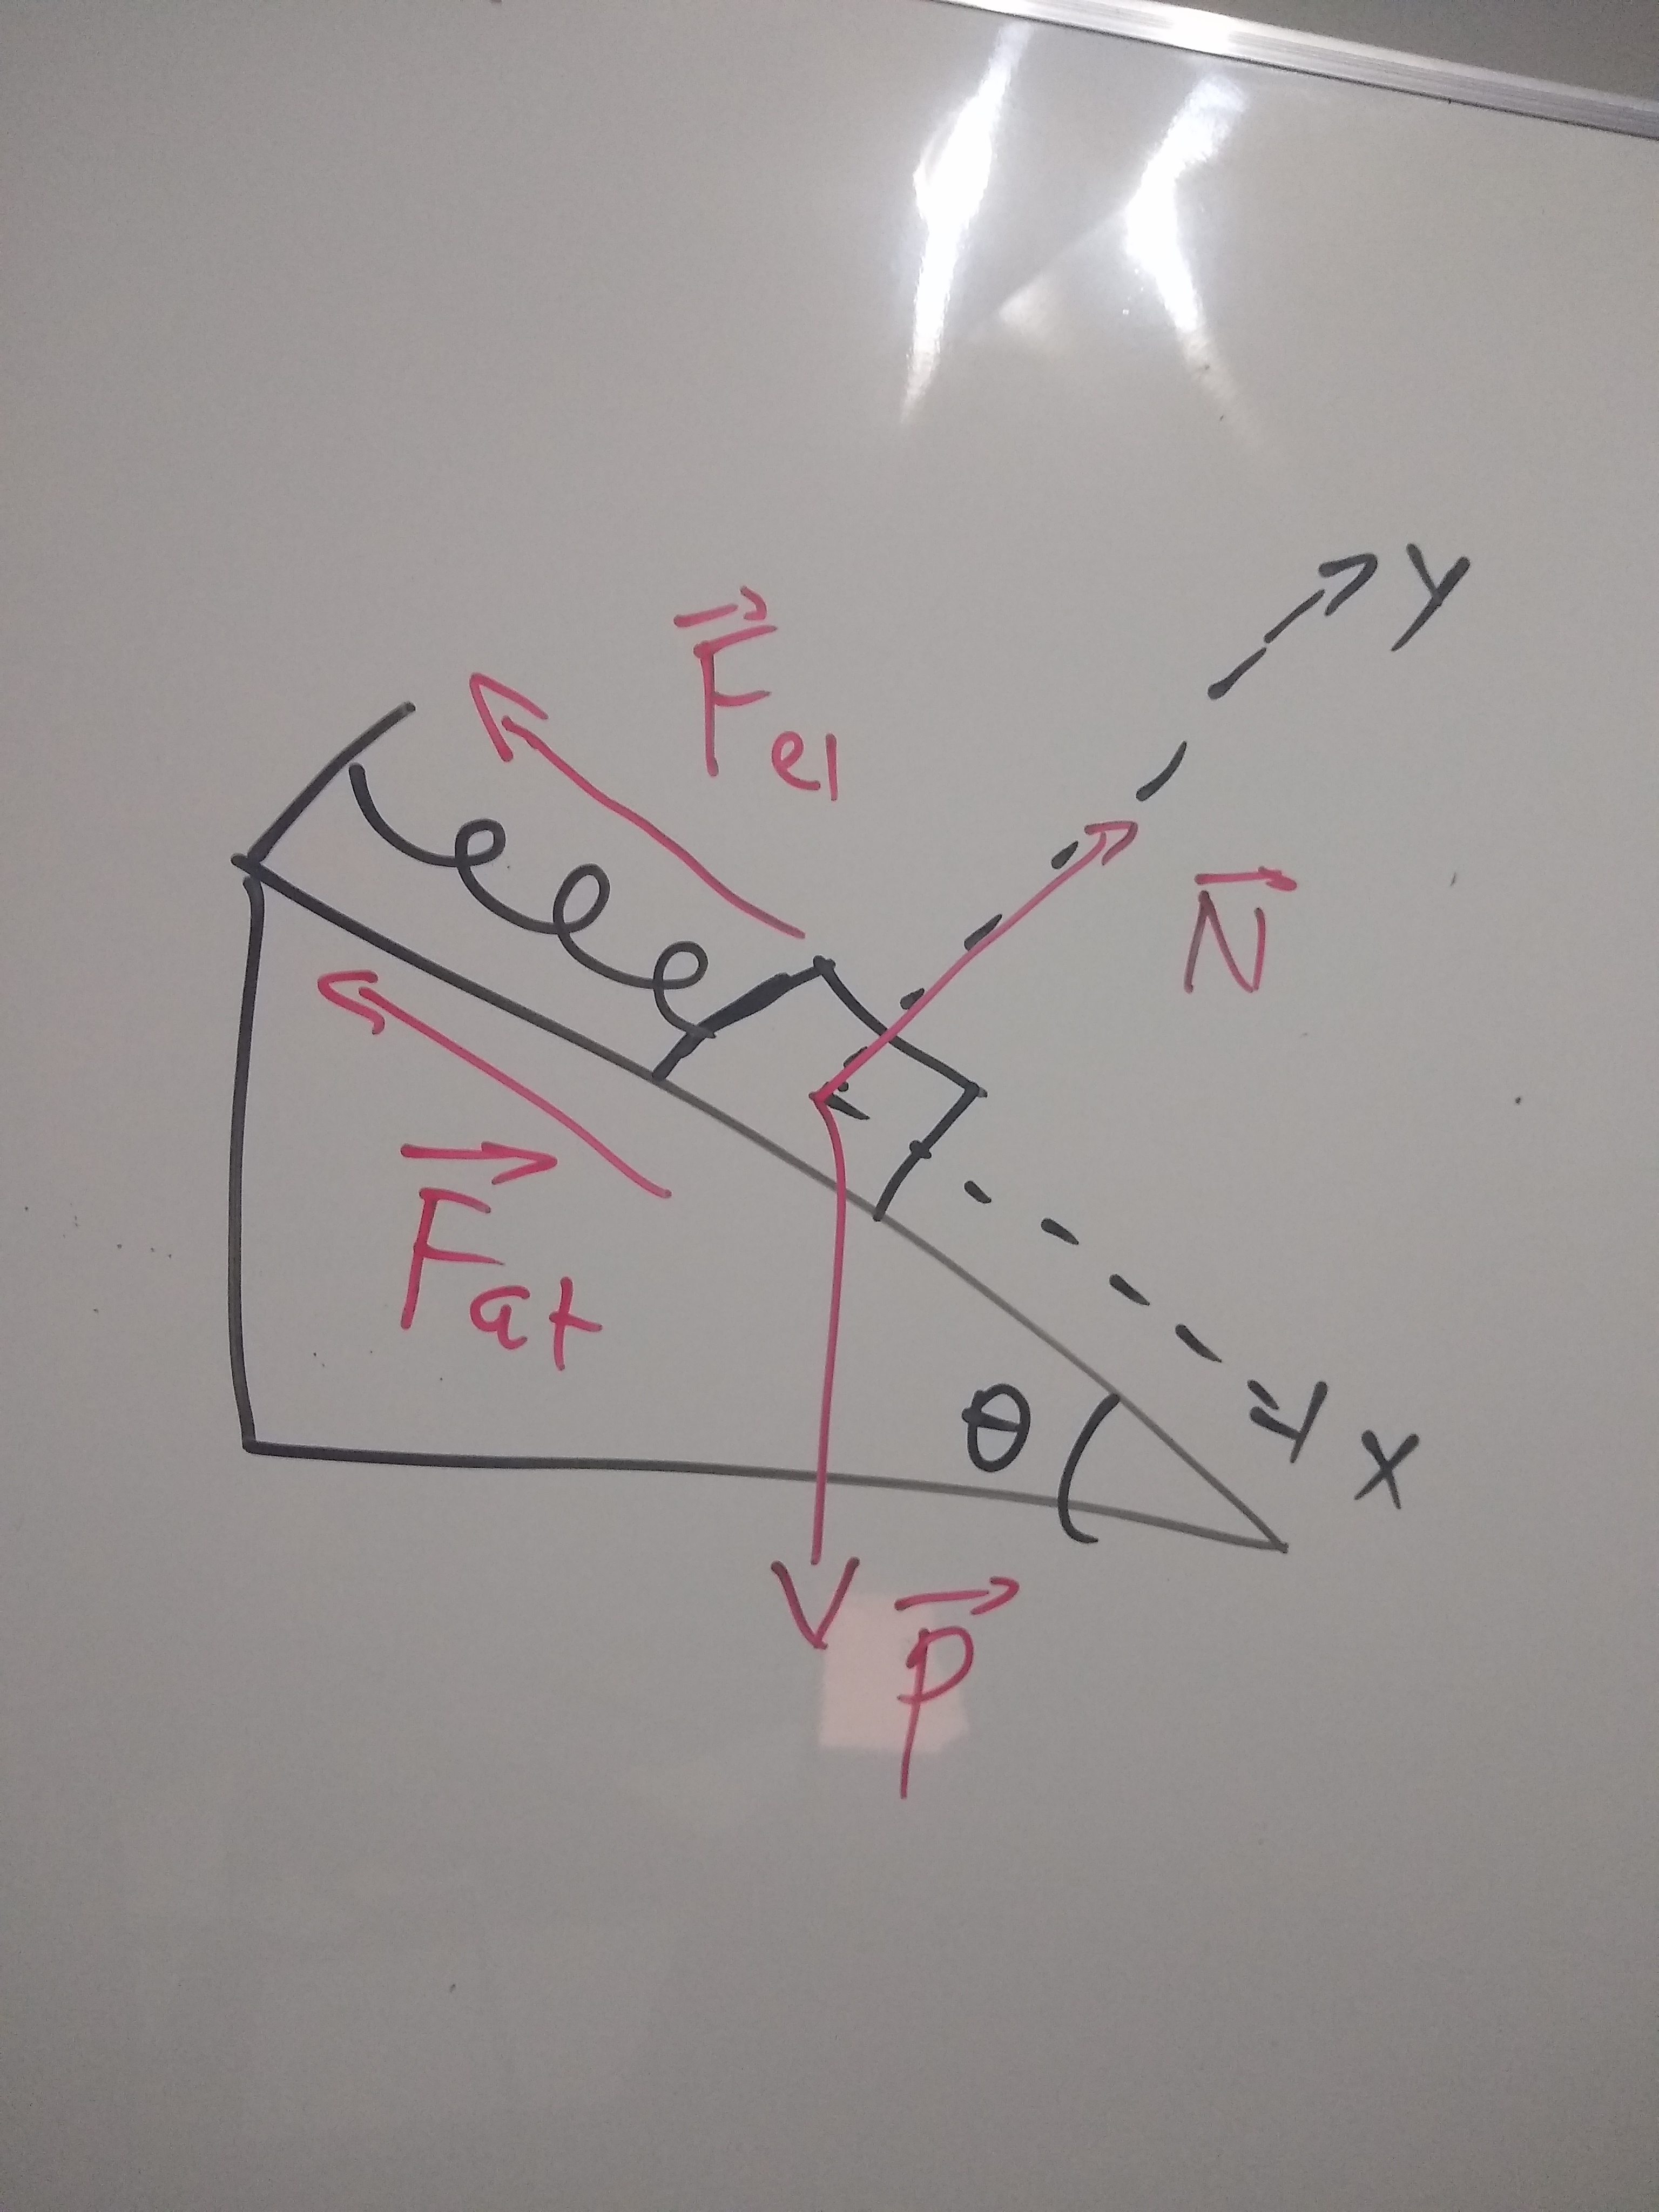
\includegraphics[width=0.4\textwidth]{plano_inclinado_mola_atrito.jpg}
    \caption{Diagrama de forças}
    \label{fig:mola_atrito}
\end{figure}

Com isso, vamos calcular as forças resultantes nas duas direções:
\begin{align*}
    &(F_{res})_{x} = P_x - F_{el} - F_{at} \\
    &(F_{res})_{y} = N - P_y =0
\end{align*}
\noindent sempre lembrando que a força resultante em y é 0, pois o bloco não se movimenta nessa direção. Analisando o caso estático (o bloco não se move) em que o atrito é limite, a força resultante na direção 'x' também é 0:
\begin{align*}
    &0=(F_{res})_{x} = mg\,sen\,\theta - k\,x - \mu\,N \\
    &0=(F_{res})_{y} = N -mg\cos\theta =0 \implies \boxed{N = mg\cos\theta}
\end{align*}
Substituindo a expressão da normal na expressão da força resultante em 'x':
\begin{align*}
    mg\,sen\,\theta - k\,x - \mu\, mg\cos\theta =0
\end{align*}
Se quisermos saber qual é a deformação que a mola sofre, isolamos o x:
\begin{align*}
    &kx = mg(sen\,\theta - \mu\,\cos\theta)\\
    &\boxed{x = \frac{mg}{k} \left(sen\,\theta - \mu\,\cos\theta\right)}
\end{align*}

\textit{Exemplo:} Um bloco de 5 kg num plano inclinado de 37$^\circ$ tem a ele acoplado uma mola de constante $k=40\,N/m$. O bloco fica totalmente em repouso durante todo o processo. O plano exerce uma força de atrito sobre o bloco também. Numa medida, viu-se que a deformação da mola é de 0,25 m. Qual é a força de atrito que o plano aplica no bloco?

\textit{Note e adote: $g=10\,m/s^2$, $sen\, 37^\circ =0,6$ e $\cos\,37^\circ = 0,8$}

\

Como o exercício quer a força de atrito e ele não diz que o atrito é o limite, então não podemos usar a fórmula da força de atrito. Então, para conseguir determiná-lo, teremos que achar via força resultante na direção 'x', que é a direção da força de atrito.

O diagrama de forças é o mesmo da figura anterior, logo a força resultante na direção 'x' é:

\begin{equation*}
    (F_{res})_{x} = P_x - F_{el} - F_{at}
\end{equation*}
Como o enunciado afirma que o bloco fica totalmente em repouso, então estamos no caso estático, o que implica que a força resultante na direção 'x' tem que ser 0. Substituindo as fórmulas nos seus lugares:
\begin{equation*}
    (F_{res})_{x} = mg\,sen\theta - kx - F_{at} =0
\end{equation*}
Substituindo os valores dados:
\begin{equation*}
    5*10*0,6 - 40*0,25 - F_{at} =0
\end{equation*}

Lembremos que $0,25 = 1/4$, então:
\begin{align*}
    &F_{at} = 30 - 40*\frac{1}{4}\\
    &F_{at} = 30 -10 \implies \boxed{F_{at} = 20\, N}
\end{align*}
\end{document}
